\subsection{Modelo insumo-produto e contas de emissões}
\label{sec:derivacao}
\label{sec:atribuicoes}

Notação
- Letras minúsicas indicam vetores coluna com 67 setores. 
- Letras maiúsculas indicam matrizes quadradas 67x67
- Chapéu indica matriz diagona. 

A MIP descreve o fornecimento de insumos entre atividades e o atendimento à demanda final. Sob coeficientes técnicos fixos, a inversa de Leontief $L$ reúne os requisitos diretos e indiretos de produção \parencite{millerBlair2009}

Da MIP são obtidos:
- a inversa de Leontief $L$, que reúne os requisitos diretos e indiretos de produção, onde cada $L_{ij}$ representa a produção de $i$ necessária por unidade monetária de demanda final de $j$.
- A produção bruta $x$ atende aos usos intermediários e à demanda final $y$.

O vetor $\widehat \varphi$ contem os coeficientes de emissão interpolados de \textcite{sanguinetAzzoni2024}.

O vetor de emissões pela ótima da produção $c$ e pela ótica da demana $u$ são dados por \parencite{marques2012}:

\begin{align}
c_i&=\varphi_i x_i, & c&=\Phi x,
\label{eq:conta-producao}
\\
u_j&=y_j\sum_i\varphi_iL_{ij}, & u&=(C\widehat y=\Phi L\widehat y)^\top\mathbf{1}.
\label{eq:conta-demanda}
\end{align}

As contas preservam o mesmo total: $c=u$. A Figura~\ref{fig:exemplo-atribuicoes} é apresentada como explo para ilustrar as contas para uma economia hipotética com 4 setores. 

% Figura vetorial copiada sem edição de:
% C:/GitHub/Mestrado/0-Projeto de Dissertação/figura_economia/contabilidade_com_sankey.pdf
% SHA-256: 861F8B5C1FDEBE3C96B31D8BD96763C2829FA2AE72703160C83949E4ACD6BF29
\begin{figure}[!htbp]
\centering
\caption{Atribuição das emissões pela produção e pela demanda em uma economia ilustrativa.}
\label{fig:exemplo-atribuicoes}
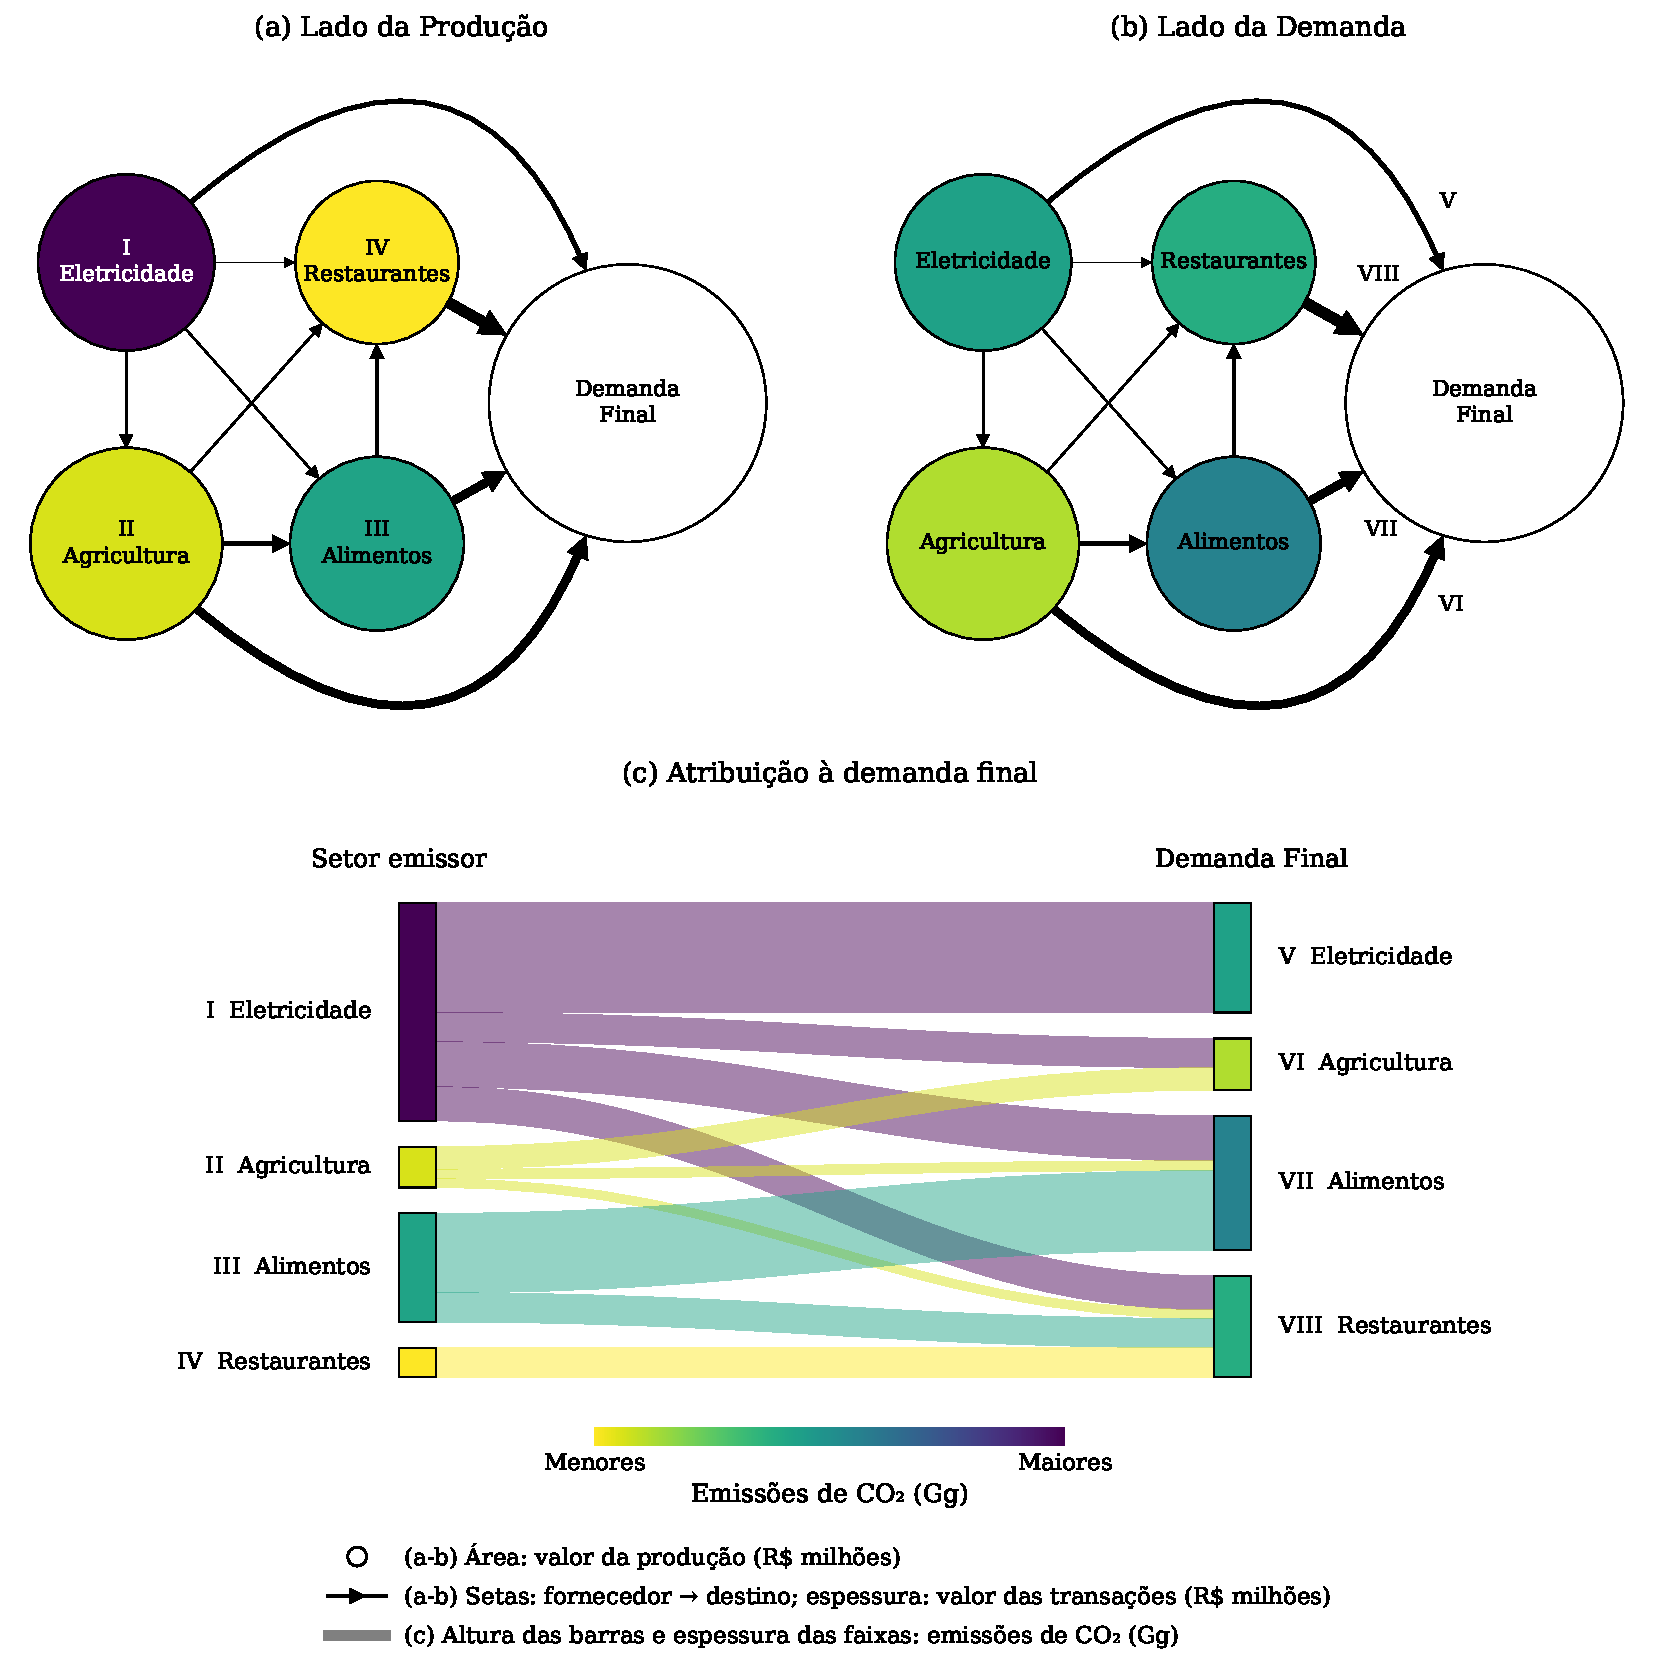
\includegraphics[width=\textwidth,height=0.76\textheight,keepaspectratio]{figuras/atribuicao_cadeia_alimentos.pdf}
\par\smallskip
\begin{minipage}{\textwidth}\footnotesize
Fonte: elaboração própria.

Nota: Exemplo de atribuição de emissões pela ótica da produção e da demanda, para uma economia hipotética de 4 setores. Em (a--b), áreas e espessuras das setas expressam valores monetários; no nó Demanda Final, a área indica o valor recebido, incluindo exportações. As cores representam $c$ em (a) e $u$ em (b). Em (c), as barras à esquerda representam as origens emissoras (I--IV) e as barras à direita, os produtos finais (V--VIII). Suas alturas e as espessuras das faixas expressam emissões em Gg de CO\textsubscript{2}. Os três quadros compartilham a escala de cores.
\end{minipage}
\end{figure}
\clearpage

